\begin{figure}
\centering
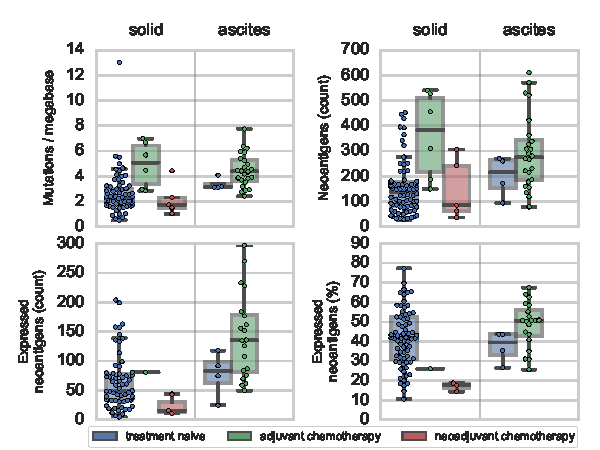
\includegraphics[scale=1.0]{figures/counts.pdf}
\caption{Mutations (upper left), neoantigens (upper right), and expressed neoantigens by count (lower left) and as a percent of total neoantigens (lower right) for samples taken before chemotherapy, after adjuvant-chemotherapy and relapse, and after neoadjuvant chemotherapy (blue, green, and red, respectively).}
\label{fig:counts}
\end{figure}

%\begin{table}[htbp]
%\begin{tabular}{lllll}
%\toprule
%{} & samples (RNA) &         Mutations &   Neoantigens & Expressed Neoantigens \\
%\midrule
%ascites pre-treatment                 &         4 (4) &  10148 $\pm$ 1000 &  199 $\pm$ 60 &           78 $\pm$ 30 \\
%ascites post-treatment                &       24 (20) &  13428 $\pm$ 1000 &  295 $\pm$ 50 &          143 $\pm$ 30 \\
%\textit{model adjusted change (\%)} &               &       57 $\pm$ 65 &   65 $\pm$ 94 &         117 $\pm$ 142 \\
%\hline
%solid pre-treatment                   &       76 (70) &    7806 $\pm$ 900 &  152 $\pm$ 20 &            63 $\pm$ 9 \\
%solid post-treatment                  &        11 (4) &  11079 $\pm$ 3000 &  264 $\pm$ 90 &           38 $\pm$ 20 \\
%\textit{model adjusted change (\%)}   &               &        6 $\pm$ 28 &   11 $\pm$ 41 &          -43 $\pm$ 35 \\
%\bottomrule
%\end{tabular}

%\caption{\textbf{Mean whole genome somatic mutations, neoantigens, and expressed noeantigens by sample type and chemotherapy treatment status.} The \textit{samples} column shows the number of samples with whole genome sequencing and, in parentheses, the number that additionally have RNA sequencing. The model-adjusted change is calculated using a Bayesian model that controls for technical variables affecting mutation identification, but does not separate treatment from coincident effects such as surgery and drift. Model effects and means are shown with 95\% credible regions and bootstrapped errors of the mean, respectively.}
%\label{tab:cohort}
%\end{table}

\begin{figure}[htbp]
\centering
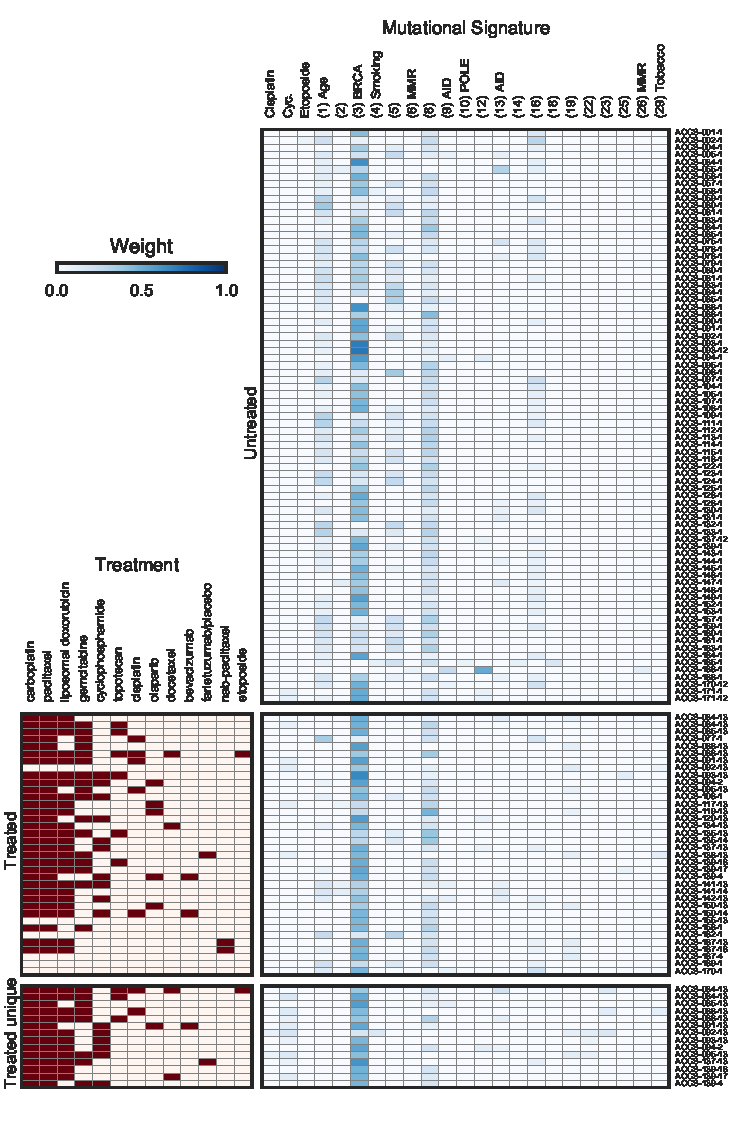
\includegraphics[scale=1.0]{figures/signatures.pdf}
\caption{\textbf{Chemotherapy treatments and detected mutational signatures for paired pre-/post-chemotherapy samples.} \textit{(Top)} Signatures detected in the pre-treatment samples. The first four signatures were extracted from reports of a \textit{G. gallus} cell line and \textit{C. Elegans} organisms after exposure to chemotherapy. COSMIC signatures numbers are shown in parentheses, and the associated mutagenic process is indicated when known. Signatures not shown were undetected in these samples. \textit{(Bottom)} Clinical treatments and detected signatures for the mutations detected only in the post-treatment samples. Cases where a chemotherapy signature is detected are annotated with a (*) if the patient received the drug and a (?) otherwise.}
\label{fig:signatures}
\end{figure}

\begin{figure}[htbp]
\centering
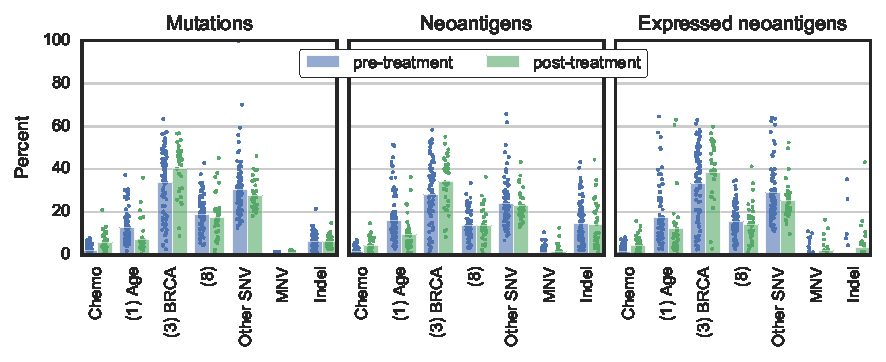
\includegraphics[scale=1.0]{figures/sources_of_mutations_and_neoantigens.pdf}
\caption{\textbf{The estimated fraction of mutations \textit{(left)}, neoantigens \textit{(center)}, and expressed neoantigens \textit{(right)} generated by SNVs from various signatures, multinucleotide variants (MNVs), and indels.} The \textit{Chemo} category sums the contributions from the chemotherapy signatures (cisplatin, cyclophosphamide, and etoposide). COSMIC signature numbers are in parentheses. The \textit{Other SNV} category shows SNVs attributed to COSMIC signatures other than the ones shown. The bars give the mean, and the points indicate individual samples.}
\label{fig:sources}
\end{figure}